\documentclass[modern]{aastex62}
\graphicspath{ {figures/} }
\DeclareGraphicsExtensions{.pdf,.eps,.png}

\usepackage{graphicx}
\usepackage{xcolor}
\usepackage{xspace}
\usepackage[sort&compress]{natbib}
\usepackage[hang,flushmargin]{footmisc}


% style tweaks
\newcommand{\acronym}[1]{{\small{#1}}}
\newcommand{\project}[1]{\textsl{#1}}
\newcommand{\code}[1]{{\texttt{#1}}}
\newcommand{\todo}[1]{\textcolor{red}{#1}}

% the following is stolen from Adrian Price-Whelan (github.com/adrn/latex-init):
\usepackage{hyperref}
\definecolor{niceblue}{rgb}{0.0, 0.4, 0.65}
\definecolor{linkcolor}{rgb}{0.02,0.35,0.55}
\definecolor{citecolor}{rgb}{0.4,0.4,0.4}
\hypersetup{colorlinks=true,linkcolor=linkcolor,citecolor=citecolor,
            filecolor=linkcolor,urlcolor=linkcolor}
\hypersetup{pageanchor=false}

% astronomy
\newcommand{\teff}{\ensuremath{T_{\rm eff}}}
\newcommand{\logg}{\ensuremath{\log g}}
\newcommand{\feh}{\ensuremath{\mathrm{[Fe/H]}}}
\newcommand{\vt}{\ensuremath{v_t}}
\newcommand{\mh}{\ensuremath{\mathrm{[M/H]}}}
\newcommand{\xh}{\ensuremath{\mathrm{[X/H]}}}
\newcommand{\I}{\textsc{I}}
\newcommand{\II}{\textsc{II}}
\newcommand{\vsini}{\ensuremath{v \sin{i}}}
\newcommand{\gcm}{\ensuremath{\mathrm{g}~\mathrm{cm}^{-3}}}
\newcommand{\kms}{\ensuremath{\mathrm{km}~\mathrm{s}^{-1}}}
\newcommand{\masyr}{\ensuremath{\mathrm{mas}~\mathrm{yr}^{-1}}}
\newcommand{\msun}{\ensuremath{\mathrm{M}_\odot}}
\newcommand{\ang}{\text{\normalfont\AA}}


\newcommand{\TF}{\code{TensorFlow}\xspace}
\newcommand{\python}{\code{python}\xspace}
\newcommand{\HARPS}{\project{\acronym{HARPS}}\xspace}
\newcommand{\HIRES}{\project{\acronym{HIRES}}\xspace}
\newcommand{\RV}{\acronym{RV}\xspace}
\newcommand{\EPRV}{\acronym{EPRV}\xspace}


% stolen from Ben Pope:
\newcommand{\kepler}{\emph{Kepler}\xspace}
\newcommand{\hipparcos}{\emph{Hipparcos}\xspace}
\newcommand{\gaia}{\emph{Gaia}\xspace}
\newcommand{\ktwo}{\emph{K2}\xspace}

% misc shortcuts
\newcommand{\flatiron}{Flatiron Institute, Simons Foundation, 162 Fifth Ave, New York, NY 10010, USA}
\newcommand{\chicago}{Department of Astronomy and Astrophysics, University of
Chicago, 5640 S. Ellis Ave, Chicago, IL 60637, USA}
\newcommand{\nyuccpp}{Center for Cosmology and Particle Physics, Department of Physics, New York University, 726 Broadway, New York, NY 10012, USA}
\newcommand{\nyucds}{Center for Data Science, New York University, 60 Fifth Ave, New York, NY 10011, USA}
\newcommand{\mpia}{Max-Planck-Institut f\"ur Astronomie, K\"onigstuhl 17, 69117 Heidelberg, Germany}


\shorttitle{Observing strategies for p-modes}
\shortauthors{bedell \textit{et al.}}

\setlength{\parindent}{1.4em} % trust in Hogg
\begin{document}\sloppy\sloppypar\raggedbottom\frenchspacing % trust in Hogg

\graphicspath{ {figures/} }
\DeclareGraphicsExtensions{.pdf,.eps,.png}

\title{Optimal Radial Velocity Observing Strategies for Solar-Like Oscillators}


\author[0000-0001-9907-7742]{Megan Bedell}
\affiliation{\flatiron}


\author[0000-0003-2866-9403]{David W. Hogg}
\affiliation{\flatiron}
\affiliation{\nyuccpp}
\affiliation{\nyucds}
\affiliation{\mpia}

\author[0000-0002-9328-5652]{Dan Foreman-Mackey}
\affiliation{\flatiron}

\author{others}

\correspondingauthor{Megan Bedell}
\email{mbedell@flatironinstitute.org}

\begin{abstract}\noindent
\todo{(this will be rewritten, probably many times!)} 
% context
Decade-scale surveys taking extreme precision radial-velocity (\EPRV)
measurements provide our best hope for finding and characterizing
truly Earth-like planets around nearby Sun-like stars.
The best \EPRV measurements are not currently limited by photon noise;
they are limited by the intrinsic variability of the target stars.
The simplest kind of variability, in some sense, is the variability
created by the fact that the target stars are, in general, pulsating
in asteroseismic pressure modes (p-modes).
% aims
Here we look at some of the practical and information-theoretic
considerations around different strategies for mitigating p-mode
noise.
% methods
We simulate the p-mode-induced intrinsic stellar surface variability
with a dynamical system that is a forest of modes, each of which is a
damped, driven harmonic oscillator, independently driven by white noise.
We consider p-mode mitigation strategies that involve choosing
sensible exposure times, including fine-tuned exposure times that
(nearly) null the dominant modes, short exposure times that resolve
the modes, and long exposure times that integrate over many mode
periods.
We consider data-analysis methods that treat the measurements as
independent measurements of the stellar velocity (simple chi-squared
fitting) and methods that model the noise as correlated in the way
that the mixture of p-mode contributions should be (kernel or
Gaussian-process methods).
% results
We find that, independent of the choice of exposure time, the
sensitivity of an \EPRV search or characterization project to
small-amplitude planet signals is improved if the data are analyzed
with an accurate p-mode noise model.
Furthermore, we find no advantage, in this data-analysis framework, to
choosing exposure times that are optimal for nulling the p-mode noise.
One limitation of these conclusions is that a good p-mode noise model
requires knowledge of the p-mode spectrum (mode frequencies and
amplitudes) this advocates taking some \EPRV or photometric data on
each target star at short enough cadences to resolve the modes; it's
a small price to pay for \emph{Earth 2.0}.
\end{abstract}

\section{Introduction}
\label{s:intro}

Modern Extreme Precision Radial Velocity (\EPRV) surveys aim for observational precisions of 0.1 \ms, corresponding to the approximate semi-amplitude of an Earth analog around a Solar analog. 
This level of precision can be achieved by instruments including \EXPRES and \ESPRESSO \citep{Petersburg2020, Pepe2021}. 
However, instrumental precision alone is insufficient to measure the Doppler signature of an Earth twin. 
The star itself contributes non-Doppler-shift radial velocity (\RV) signals due to its intrinsic variability, and these effects must be mitigated in some way. 
Modern observing programs are therefore engineered to minimize the contributions of such signals to the final \RV time series.

One significant source of stellar noise for \EPRV is asteroseismic oscillations. 
For a Sun-like star, the most observable asteroseismic oscillations are \textit{p-mode} signals with a characteristic period of around 5 minutes and an amplitude on the order of 1 \ms. 
Unlike some types of stellar activity, p-mode oscillations \textit{are} Doppler shifts arising from the radial motion of the stellar surface, so advanced methods of disentangling non-Doppler spectral distortions from the measured \RV will have very limited effect. 
On the other hand, asteroseismic oscillations are physically well-understood and relatively simple to model, unlike other \RV noise sources. 
Both of these factors make them a somewhat unique term in the \EPRV error budget.

The default approach to minimize the influence of p-modes in \EPRV observations is integrating for 10 minutes or more \citep{Dumusque2011}. 
This is intended to average over a couple cycles of the (approximately sinusoidal) oscillation signal. 
If the star is bright enough to saturate the detector during a long integration, as a significant number of prime \EPRV targets are, multiple short exposures may be taken and binned. 

More recently, \citet[][hereafter C19]{Chaplin2019} put forward the alternative of setting each target's integration time to be a multiple of the individual star's expected oscillation period. 
This optimal exposure time approach still aims to average over the stellar oscillation signal, but it is more robust than an arbitrarily chosen exposure duration in the regime of short exposure times. 
For example, as demonstrated by C19 with synthetic data, an exposure time of 10 minutes is actually pessimal for the Sun-like star $\alpha$~Cen~B. 
This is because 10 minutes is close to 1.5 times the characteristic oscillation period of the star, which leaves significant asteroseismic noise in the integrated \RV observations. 
The best choices of exposure time are either an integer multiple of the oscillation period (to integrate over the cycle effectively) or a much longer exposure encompassing $N>>1$ cycles (to achieve a $\sqrt{N}$ reduction in noise). 
Thus, when aiming for \RV precision of 0.1 \ms\ and simultaneously trying to observe targets efficiently (\ie not integrating for hours on an individual target), an exposure time tailored to the individual target's oscillation period is required to deal with asteroseismic noise.

Even with an optimally-chosen exposure time, there are some drawbacks to integrating over the asteroseismic oscillations. 
For one thing, the nulling approach will always be limited by the stochastic nature of the oscillations. 
\todo{(say more)} 

There is also a case to be made that asteroseismic oscillations contain valuable scientific information. 
Asteroseismology is the only means of observationally constraining the interior composition of stars, and it can provide high-precision estimates of properties like stellar age and mass. 
Asteroseismology of solar-like oscillators with ground-based \RV data is a well-established field \citep[see e.g.][for a review]{Bedding2003}, but it has been largely incompatible with \RV planet-hunting due to the explicit aim of nulling the asteroseismic signals in exoplanet detection experiments. 
However, the stellar properties inferred in asteroseismology are also important to studies of exoplanets, so it would be beneficial to \EPRV surveys to preserve asteroseismic information if it can be done without too much cost to the planetary signals.

In this work, we explore the alternative approach of \textit{resolving} and \textit{modeling} asteroseismic signals in \EPRV observations. 


We use a combination of realistic simulations and actual \EXPRES data to explore the potential benefits of observing strategies for \EPRV which resolve stellar p-mode oscillations. 


\section{Simulated Data}

Stellar p-mode oscillations are well-approximated as a set of damped driven simple harmonic oscillators \todo{(citation needed)}. 
These independent oscillators have their characteristic frequencies and amplitudes set by the seismic power spectrum, which resembles a comb of frequencies centered on \numax\ and separated by \deltanu.

Using this framework, we simulate solar-like oscillations as a dense grid of velocities. 
\todo{(MATH HERE)}
\todo{(INSERT FIGURE OF POWER SPECTRUM)}

From this dense grid, we can derive \RV observations with any choice of start time and exposure length by averaging the velocities within that window of observation. 
As an illustrative example, we show three different choices of observing times in Figure \ref{fig:binning-sim}. 
\todo{(more -- return to point of stochasticity from intro)}

\begin{figure}
    \centering
    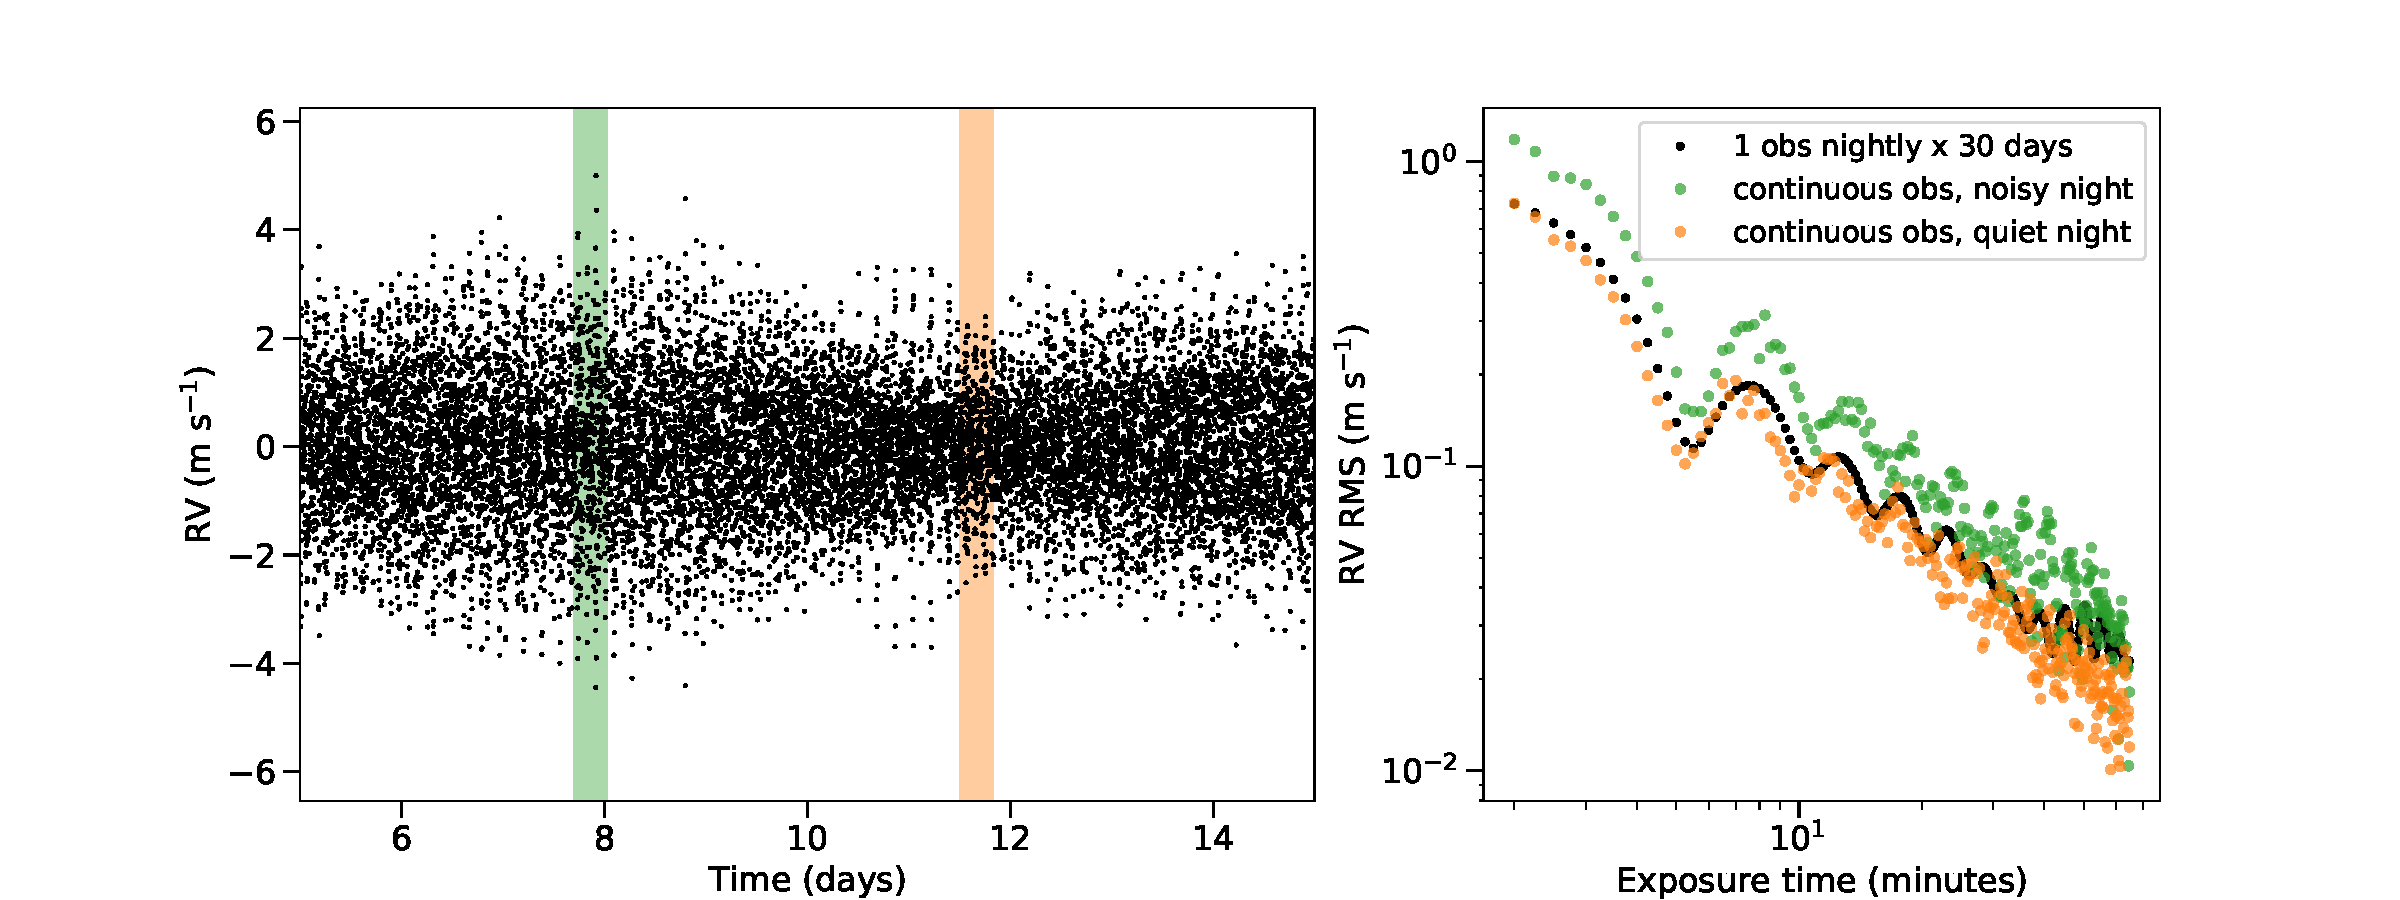
\includegraphics{figures/binning_test.pdf}
    \caption{\todo{caption}}
    \label{fig:binning-sim}
\end{figure}




\begin{itemize}
\item Power spectra used: simple solar-like oscillator with p-modes only and with granulation too
\item (two-panel plot of power spectra)
\item How WF's GP model works
\item Timestamps of observations
\item (two-panel plot of full, noise-free observations)
\item Making these into realistic observations: how we handle binning + noise injections (both photon + read noise)
\end{itemize}

\section{Observing Strategies}

\subsection{Long Exposures}

Test performance of integrating over p-modes. Show that due to stochasticity, an ``optimal'' exposure time isn't always optimal.

\subsection{Short Exposures}

Test performance of resolving p-modes. Say some things about Nyquist limits to motivate choice of exposure times.

\begin{itemize}
\item Functional form of model used
\item Performance in several regimes of read noise/read-out time
\item Does this still work with granulation included?
\end{itemize}

\subsection{Hybrid Strategies}

???

\section{Validation on Real Data}

\HARPS observations of asteroseismic star -- probably 18 Sco \citep{Bazot2012}.

\section{Discussion}

Recommendations for observers.

Potential limitations -- will other noise sources leak in? Is there any chance that this will bias recovery of planet signals?

Need to know mode spectrum

The possibility that there are Teff variations that are observable.

\acknowledgements

The authors thank
  Ben Pope (Queensland),
  Will Farr (Flatiron),
  Rodrigo Luger (Flatiron),
  Simon J. Murphy (Sydney),
  Didier Queloz (Cambridge), and
  Lily Zhao (Yale)
for useful conversations.

\software{
    \code{Astropy} \citep{astropy},
    \code{IPython} \citep{ipython},
    \code{matplotlib} \citep{matplotlib},
    \code{numpy} \citep{numpy},
    \code{scipy} (\url{https://www.scipy.org/}),
}

% \facility{}

\clearpage
\bibliographystyle{aasjournal}
\bibliography{ms}

\end{document}
